\chapter{CoAP library module} \label{coaplibrary}

In hoofdstuk \ref{CoAP} bekeken we beknopt hoe het CoAP protocol in mekaar zit en wat er allemaal mogelijk is. In dit hoofdstuk bekijken we hoe een eigen CoAP library in PHP werd ontwikkeld als Drupal module. De module stelt een Drupal gebruiker in staat CoAP berichten op te stellen, te versturen en te ontvangen. Let wel, deze module heeft niet als doel om visueel iets voor te stellen op een website. Ze is slechts functioneel en bijvoorbeeld te gebruiken in een andere module die dan de berichten kan omvormen tot een visuele representatie. Dit laatste is wat wij doen in de uiteindelijk te ontwerpen module welke wordt toegelicht in hoofdstuk \ref{resourcemodule}.

\section{Doel}

Wanneer we trachtten CoAP berichten op te stellen, te versturen en ontvangen in onze module, werd al snel het nut duidelijk van een aparte module die zou fungeren als CoAP library. Er ontstaat namelijk erg veel duplicatie van code, bovendien wordt de code onoverzichtelijk en slordig. Nog een zeer nadelig gevolg is dat de code niet hergebruikt kan worden in een andere module. Men zou al de code moeten doorspitten om net dat stuk te vinden waar CoAP gesproken wordt. Bovendien is het niet zeker dat die code zal voldoen aan de waarschijnlijk andere eisen van de nieuwe gebruiker. Wanneer de code niet fungeert in de nieuwe situatie, zal er veel tijd gespendeerd worden aan debuggen en zal de frustratie oplopen bij de gebruiker. Kortom, het is duidelijk dat dit een zeer slechte praktijk is die ten alle kosten moet vermeden worden, het druist in tegen enkele van de belangrijkste programmeerprincipes.\\

Met het nut bewezen bekijken we even wat een gebruiker van deze library moet kunnen verwachten. Ze moet de gebruiker in staat stellen dynamisch berichten op te stellen, volledig naar eigen wens. Dit wil zeggen dat de verzameling operaties om een bericht op te stellen, alle mogelijke berichten moet kunnen genereren. Dit heeft als gevolg dat elke elementaire operatie moet kunnen worden uitgevoerd op een bericht. Opstellen van bijvoorbeeld een bepaald bericht aan de hand van slechts één functie is niet prioritair en dus bijkomstig. Het is uiterst belangrijk bij het ontwerp van deze library dat de gebruiker zich niet meer moet bekommeren technische details zoals hexadecimale code die nodig is in een bericht. Alle technische details zitten verborgen in de CoAP library module. We besluiten dat de library een gebruiker in staat moet stellen dynamisch en gebruiksvriendelijk berichten op te stellen, en dit met een minimum aan code.

\subsection{Essenti\"{e}le, te ondersteunen functies} \label{essentielefuncties}

We sommen enkele van de eerder vermelde elementaire functies op, deze opsomming is allesbehalve limitatief:

\begin{itemize}
\item Opstellen van de header en token waarbij de gebruiker het type, de methode en het token opgeeft. De token lengte wordt afgeleid uit het token. Wanneer geen token gewenst is, kan de gebruiker een lege string meegeven.
\item Een optie toevoegen aan het bericht waarbij de gebruiker slechts het optienummer en de waarde van de optie moet meegeven. De gebruiker hoeft zich hierbij geen zorgen te maken over het mechanisme waarbij de Option Delta gebruikt wordt, of over de lengte van de waarde, noch over de volgorde van de opties. Evenmin moet de gebruiker rekening houden met het feit dat wanneer de Option Delta of lengte van de waarde groter is dan 12, een mechanisme met extra bytes wordt gebruikt.
\item De payload toevoegen aan het bericht waarbij de gebruiker slechts de payload hoeft op te geven.  Dit houdt in dit geval in dat de payload marker wordt toegevoegd en dat de lengte van de payload wordt afgeleid uit de payload zelf.
\item Een bericht versturen, hierbij onderscheiden we 2 mogelijkheden:
\begin{itemize}
\item Het sturen van een bericht zonder observe optie: Hierbij hoeft men enkel rekening te houden met \'{e}\'{e}n antwoord. Men kan dus het antwoord teruggeven als return waarde van de functie die het bericht stuurt. Men hoeft zich niet te bekommeren om meerdere antwoorden die op willekeurige tijdstippen kunnen aankomen.
\item Het sturen van een bericht met observe optie: Het antwoord dat hierop terug gestuurd wordt, bevat slechts \'{e}\'{e}n waarde en is slechts een bevestiging dat de server de client heeft toegevoegd aan de lijst van ge\"{i}nteresseerden. De server zal nu op vaste tijdstippen een antwoord sturen op eigen initiatief. Er moet dus een mechanisme voorzien worden dat het aankomen van die berichten opvangt. We zullen later in dit hoofdstuk zien (zie \ref{observe_hooks}) hoe we deze probleemstelling in de library hebben opgevangen.
\end{itemize}
Hierbij wordt de gebruiksvriendelijkheid doorgetrokken, de gebruiker staat namelijk niet in voor de controle van de aanwezigheid van een observe optie. Dit wordt automatisch gedetecteerd door de CoAP library.
\item Operaties om een bericht te ontmantelen, hieronder verstaan we het parsen van onder andere de payload, een optie op basis van optienummer, het message ID, het token, ...
\end{itemize}

Merk op dat bij het genereren van CoAP berichten ook een message ID nodig is. Ook hierop is de CoAP library voorzien, er wordt bijgehouden welke message ID's al gebruikt zijn door telkens het laatst gebruikte message ID te incrementeren. Dit is een mechanisme dat aangeraden wordt in de CoAP draft (versie 14).\\
Een soortgelijk principe wordt toegepast wanneer een token moet worden gegenereerd. De gebruiker moet dan wel een lengte aangeven.\\
Ook wanneer een ACK of RST moet worden gegenereerd wordt, door aan te geven op welk bericht het antwoord moet worden gestuurd, automatisch het message ID uit het oorspronkelijk bericht geparsed en in het antwoord geplaatst. Hetzelfde principe geldt wanneer een token moet worden overgenomen.

\subsection{Optionele, handige functies} \label{optionelefuncties}

Sommige berichten zijn vaker nodig dan andere. Om de gebruiksvriendelijkheid van de library te verhogen en de drempel om ze te gebruiken te verlagen, is het een goed idee enkele functies te voorzien om bepaalde volledige berichten op te stellen. Belangrijk hierbij is dat deze opgestelde berichten nog steeds aanpasbaar moeten zijn. Dit zorgt ervoor een gebruiker bijvoorbeeld al een basisbericht kan opstellen en het daarna nog naar eigen wens kan aanpassen, wat de gebruiker veel tijd bespaart. We geven enkele voorbeelden die ook ge\"{i}mplementeerd zijn in de library, deze opsomming is alweer niet limitatief:
\begin{itemize}
\item Opstellen van een basis GET request: hierbij krijgt de gebruiker meteen de kans om een URI-path optie toe te voegen aan het bericht. De gebruiker hoeft hier enkel het desbetreffende URI-path toe te voegen. De optie wordt automatisch toegevoegd door de library op basis van de invoer. Wanneer de gebruiker geen URI-path meegeeft, wordt er ook geen optie toegevoegd aan het bericht.
\item Opstellen van een basis GET request met observe optie: deze operatie is zeer vergelijkbaar met de vorige, het enige verschil is dat er een lege observe optie wordt toegevoegd. Dit zorgt ervoor dat de server waarnaar het bericht wordt verstuurd, de client zal toevoegen aan de lijst met ge\"{i}nteresseerden. Om de goede programmeerprincipes te volgen wordt in deze operatie gebruik gemaakt van de vorige operatie. Dit om duplicatie van code te vermijden.
\item Automatisch genereren van een ACK op basis van een opgegeven bericht: de gebruiker hoeft enkel het bericht mee te geven waarop de ACK moet worden opgesteld. Het message ID wordt automatisch overgenomen uit het oorspronkelijk bericht. Naast het feit dat de gebruiksvriendelijkheid verhoogd wordt, heeft deze operatie nog een niet te verwaarlozen nut. De kans op fouten wordt namelijk veel kleiner omdat de ACK automatisch gegenereerd wordt, menselijke fouten zijn dus zo goed als uitgesloten als deze operatie op punt staat.
\item Automatisch genereren van een RST op basis van een opgegeven bericht: deze operatie is volledig analoog aan de vorige met dat verschil dat het type van dit bericht RST is in plaats van ACK.
\end{itemize}

\section{Implementatie}

In deze paragraaf wordt besproken hoe de library effectief ge\"{i}mplementeerd werd. De volgorde van de subparagrafen is tevens chronologisch. 

\subsection{Proceduregericht}

De eerste versie van de CoAP library werd proceduregericht geprogrammeerd. Dit houdt in dat geen staten of objecten bijgehouden worden. Bijgevolg moet de gebruiker zelf het bericht bijhouden onder een vorm die hij/zij zelf kiest. Deze versie van de CoAP library verwachtte echter het bericht onder de vorm van een hexadecimale string. Alle benodigde operaties die eerder vermeld werden, werden ge\"{i}mplementeerd. Alhoewel deze eerste versie al zeker een stap in de goede richting was, zijn er toch wel enkele nadelen die de kop opsteken. Zoals eerder al vermeld, is de gebruiker verplicht zelf de hexadecimale string bij te houden die het bericht voorstelt. Niet elke gebruiker is bekend met het gebruik van hexadecimale strings. Een tweede nadeel heeft te maken met bescherming van het bericht. Wanneer de gebruiker de hexadecimale string bijhoudt, kan die worden aangepast naar believen. Het bericht kan zo vervormd en mogelijks nutteloos worden. Bovendien kan de gebruiker zonder het te beseffen het bericht door \'{e}\'{e}n of andere operatie omvormen tot een normale string met American Standard Code for Information Interchange (ASCII)-karakters \nomenclature{ASCII}{American Standard Code for Information Interchange}. Dit heeft mogelijk als gevolg dat de library het bericht zal omvormen tot een verkeerde hexadecimale string. Kortom, er is nog ruimte voor verbetering en een objectgerichte implementatie lijkt voor de hand liggend.

\subsection{Objectgericht}

In de vorige subparagraaf zagen we de nadelen van een proceduregerichte oplossing. Het zijn net deze punten waar een objectgerichte oplossing goed op scoort. De tweede versie van de CoAP library maakt gebruik van twee klassen welke besproken worden in volgende puntjes.

\subsubsection{CoAPFactory klasse}

Zoals de naam al suggereert, wordt deze klasse gebruik voor generatie van CoAP berichten. De gebruiker maakt eerst een instantie aan van de CoAPFactory klasse. Dit object kan dan gebruikt worden om CoAP berichten aan te maken. Het is deze klasse die de eerder besproken handige functies (zie \ref{optionelefuncties}) implementeert om bepaalde berichten aan te maken, samen met de operatie die de header en token opstelt. Alle operaties die een berichtobject aanmaken geven een object terug van klasse CoAPMessage, deze klasse wordt hierna besproken. De constructor van deze factory klasse ontvangt volgende parameters:
\begin{itemize}
\item Modulenaam: deze parameter bevat de naam van de module die gebruik maakt van de CoAP library, de reden voor deze parameter wordt hierna uitgelegd in subparagraaf \ref{observe_hooks}.
\item IPv6-adres: deze parameter bevat een geldig IPv6-adres, dit is het IPv6-adres van het embedded device waarop de beoogde resource is aangesloten.
\item URI-path: deze parameter bevat een URI-path van een resource op het embedded device dat aangegeven wordt door het IPv6-adres. Deze parameter mag achterwege gelaten worden, het URI-path is dan leeg en duidt het embedded device zelf aan.
\end{itemize}
Zoals blijkt uit de parameters wordt een factory per gewenste resource aangemaakt.

\subsubsection{CoAPMessage klasse}

Deze klasse representeert het bericht zelf. Het bevat ten allen tijde het bericht in hexadecimale vorm. Het is deze klasse die de essenti\"{e}le operaties (zie \ref{essentielefuncties}) implementeert op het opstellen van de header en token na, zodanig dat het bericht kan worden aangepast naar eigen wensen en noden. Het bericht kan dan gemakkelijk worden verstuurd door een send-operatie op het object uit te voeren. Een IPv6-adres opgeven hoeft niet meer, dit is reeds gebeurd bij constructie van de factory die dit bericht heeft aangemaakt. Aangezien CoAP werkt met UDP, moet er een UDP socket geopend worden. Bovendien moet in het geval de observe functionaliteit gebruikt wordt, de socket onderhouden worden. Daar berichten later kunnen toekomen op initiatief van de server.

\subsection{Hooks voor notificaties} \label{observe_hooks}

Eerder werd al aangehaald dat er een speciale voorziening nodig is voor de observe functionaliteit. Hierbij kan de server op eigen initiatief notificaties sturen naar ge\"{i}nteresseerde clients. Enkele alternatieven werden bedacht en overwogen, het een al beter dan het ander:
\begin{itemize}
\item Socket teruggeven: Dit houdt in dat de send-functie die opgeroepen wordt in de CoAP library als return waarde de socket zou teruggeven. Dit heeft echter als gevolg dat een gebruiker verder zelf de socket moet onderhouden en telkens de nodige berichten moet opbouwen, versturen en ontvangen. Het spreekt voor zich dat dit geen goede oplossing is. De CoAP library wordt zo allesbehalve modulair en een eventuele gebruiker ervan moet al een redelijke hoeveelheid technische kennis hebben om ze te gebruiken.
\item Databank: bij dit alternatief zou men de socket toch beheren in de CoAP library zelf en de notificaties opslaan in de databank. Men kan dan bijvoorbeeld een gebruiker van de module een naam van een databanktabel laten opgeven en de notificaties daarin opslaan. Dit is al een betere oplossing, maar deze heeft ook wel wat nadelen. Er is namelijk geen enkele controle mogelijk of de kolommen van de databank wel kloppen en nog belangrijker, of de tabel wel bestaat. Ook is er nu niet echt sprake van abstractie, de gebruiker moet zich aanpassen aan de library. Bovendien moet de gebruiker kennis hebben over het gebruik van een databank, wil hij de library gebruiken.
\item Hook mechanisme: Dit is het laatste en door ons gekozen alternatief. De CoAP library definieert hierbij 3 hooks die een gebruiker moet implementeren. \'{E}\'{e}n van de voordelen hiervan is dat de Drupal ontwikkelaar normaal gezien al bekend is met het hook mechanisme van Drupal zelf. Het gebruikte mechanisme is namelijk analoog, de hook wordt ge\"{i}mplementeerd door het woord hook te vervangen door de naam van de module. Deze moeten ge\"{i}mplementeerd worden maar ze mogen leeg zijn. We sommen even de te implementeren hooks op:
\begin{itemize}
\item \textit{hook\_receive\_response}: Deze hook wordt opgeroepen telkens wanneer een notificatie binnen komt. De CoAP library bouwt een response-object op van de klasse CoAPMessage en geeft deze mee als argument met de hook. Zo kan de gebruiker zelf beslissen wat er met het antwoord moet gebeuren. Men kan zo spreken van een hoge mate van abstractie.
\item \textit{hook\_receive\_error}: Wanneer een fout gebeurt, bijvoorbeeld een sensor die laat of zelfs niet meer reageert, wordt deze hook opgeroepen. Als argumenten worden de foutboodschap, het IPv6-adres en URI-path van de resource meegegeven. Alweer kan de gebruiker van de library zelf beslissen wat er met deze foutboodschap moet gebeuren.
\item \textit{hook\_stop\_observers}: Wanneer een observe op een resource stopt, om welke reden dan ook, wordt deze hook opgeroepen. Dit biedt een gebruiker van de library de kans om de consistentie van de eigen module te behouden en fouten te vermijden. Men kan bijvoorbeeld melden op een eventueel gemaakt website dat de observe gestopt is. Als parameters worden het IPv6-adres en het URI-path van de resource meegegeven zodat de gebruiker weet over welke resource het gaat.
\end{itemize}
\end{itemize}

We merken verder nog op dat de CoAP library zelf instaat voor het bijhouden van de te observeren resources. Bovendien wordt om de resource zo weinig mogelijk te belasten, slechts \'{e}\'{e}n observe uitgevoerd op de resource, ongeacht hoeveel gebruikers erin ge\"{i}nteresseerd zijn. Een observe wordt pas gestopt wanneer geen enkele gebruiker meer ge\"{i}nteresseerd is in de resource.

% HIER VERDERWERKEN

\subsection{Opvangen van verloren berichten}

Omdat het CoAP protocol gebruik maakt van UDP kunnen pakketten verloren gaan, dit moet dus opgevangen worden indien CON berichten verstuurd worden. In de CoAP draft (versie 14) wordt exponential backoff voorgeschreven. In de CoAP library werd die geïmplementeerd met de standaardwaarden die eveneens in de CoAP draft (versie 14) staan. Het principe is dat wanneer geen ACK ontvangen wordt als antwoord op het CON bericht, het CON bericht opnieuw verstuurd wordt met daartussen exponentieel stijgende perioden tot een ACK ontvangen wordt of een maximum aantal verzendingen overschreden wordt. Hiervoor moeten 2 dingen worden bijgehouden: een timeout waarde en een retransmition counter die bijhoudt hoeveel keer het CON bericht al opnieuw werd verstuurd. De timeout waarde wordt ge\"{i}nitialiseerd op een random waarde tussen ACK\_TIMEOUT en ACK\_TIMEOUT*ACK\_RANDOM\_FACTOR, ACK\_TIMEOUT en ACK\_RANDOM\_FACTOR zijn constanten. De retransmission counter wordt initieel ingesteld op 0. Wanneer de timeout overschreden wordt en de retransmission counter nog steeds een waarde bevat die kleiner is dan MAX\_RETRANSMIT (nog een constante), wordt het CON bericht opnieuw verzonden en de timeout waarde verdubbeld. De constanten werden in de CoAP library ingevuld met volgende waarden die voorgeschreven worden in de CoAP draft (versie 14):
\begin{itemize}
\item \textit{ACK\_TIMEOUT}: 2 seconden
\item \textit{ACK\_RANDOM\_FACTOR}: 1,5
\item \textit{MAX\_RETRANSMIT}: 4
\end{itemize}

%ALLES HIERNA HOORT HIER NIET THUIS, MAAR WEL ELDERS

%\section{Architectuur}

%\subsection{Functionaliteit}

%Hier komt de functionaliteit van de CoAP library.\\

%Een van de belangrijkste aspecten bij deze masterproef is een minimale belasting te realiseren voor de sensoren, dit is immers de reden voor de ontwikkeling van CoAP. Opgehaalde waarden %zullen dan ook in de databank worden opgeslagen met een geldigheidswaarde, wanneer een waarde nog geldig is, wordt de waarde uit de databank gehaald en wordt het embedded device niet %opnieuw bevraagd. Slechts wanneer de waarde niet meer geldig is, wordt het embedded device aangesproken.\\

%\subsection{Content-type in de databank}

%Wanneer data ontvangen wordt, moet deze opgeslagen worden in de databank. Er moet dan ook een tabel voorzien worden in de databank met de nodige velden, het content-type in de databank:

%\begin{wrapfigure}{r}{0.3\textwidth}
%\vspace{10pt}
%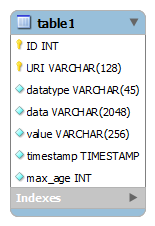
\includegraphics[width=0.3\textwidth]{fig/contentTypeDatabank}
%\vspace{-35pt}
%\caption{Content-type in databank}
%\vspace{-10pt}
%\end{wrapfigure}
%\paragraph{}
%\vspace*{-\parskip}

%\begin{itemize}
%\item Een ID van de resource,
%\item de URI van het embedded device,
%\item het datatype van de ontvangen waarde (XML, JSON, plain text, etc),
%\item de effectieve data (originele, raw input),
%\item de verwerkte data,
%\item een timestamp die het tijdstip van opvragen aanduidt,
%\item waarde om de geldigheid te controleren (max age).
%\end{itemize}
